\documentclass[10pt,a4paper]{article}
\usepackage[utf8]{inputenc}
\usepackage[french]{babel}
\usepackage[T1]{fontenc}
\usepackage{amsmath}
\usepackage{amsthm}
\usepackage{amsfonts}
\usepackage{amssymb}
\usepackage{graphicx}
\usepackage{mathrsfs}
\usepackage{url}
\usepackage{color}
\usepackage{listings}
\definecolor{mygreen}{RGB}{28,172,0} % color values Red, Green, Blue
\definecolor{mylilas}{RGB}{170,55,241}
\lstset{language=Matlab,%
%basicstyle=\color{red},
breaklines=true,%
morekeywords={matlab2tikz},
keywordstyle=\color{blue},%
morekeywords=[2]{1}, keywordstyle=[2]{\color{black}},
identifierstyle=\color{black},%
stringstyle=\color{mylilas},
commentstyle=\color{mygreen},%
showstringspaces=false,%without this there will be a symbol in the places where there is a space
numbers=left,%
numberstyle={\tiny \color{black}},% size of the numbers
numbersep=9pt, % this defines how far the numbers are from the text
emph=[1]{for,end,break},emphstyle=[1]\color{red}, %some words to emphasise
%emph=[2]{word1,word2}, emphstyle=[2]{style},    
}
\lstset{literate=
{á}{{\'a}}1 {é}{{\'e}}1 {í}{{\'i}}1 {ó}{{\'o}}1 {ú}{{\'u}}1
{Á}{{\'A}}1 {É}{{\'E}}1 {Í}{{\'I}}1 {Ó}{{\'O}}1 {Ú}{{\'U}}1
{à}{{\`a}}1 {è}{{\`e}}1 {ì}{{\`i}}1 {ò}{{\`o}}1 {ù}{{\`u}}1
{À}{{\`A}}1 {È}{{\'E}}1 {Ì}{{\`I}}1 {Ò}{{\`O}}1 {Ù}{{\`U}}1
{ä}{{\"a}}1 {ë}{{\"e}}1 {ï}{{\"i}}1 {ö}{{\"o}}1 {ü}{{\"u}}1
{Ä}{{\"A}}1 {Ë}{{\"E}}1 {Ï}{{\"I}}1 {Ö}{{\"O}}1 {Ü}{{\"U}}1
{â}{{\^a}}1 {ê}{{\^e}}1 {î}{{\^i}}1 {ô}{{\^o}}1 {û}{{\^u}}1
{Â}{{\^A}}1 {Ê}{{\^E}}1 {Î}{{\^I}}1 {Ô}{{\^O}}1 {Û}{{\^U}}1
{œ}{{\oe}}1 {Œ}{{\OE}}1 {æ}{{\ae}}1 {Æ}{{\AE}}1 {ß}{{\ss}}1
{ű}{{\H{u}}}1 {Ű}{{\H{U}}}1 {ő}{{\H{o}}}1 {Ő}{{\H{O}}}1
{ç}{{\c c}}1 {Ç}{{\c C}}1 {ø}{{\o}}1 {å}{{\r a}}1 {Å}{{\r A}}1
{€}{{\euro}}1 {£}{{\pounds}}1 {«}{{\guillemotleft}}1
{»}{{\guillemotright}}1 {ñ}{{\~n}}1 {Ñ}{{\~N}}1 {¿}{{?`}}1
}
\usepackage[french,onelanguage,ruled,lined,linesnumbered]{algorithm2e}
\SetKw{And}{et}
\SetKw{From}{allant de}
\author{\textsc{TRAN Quoc Nhat Han} \& \textsc{Adrien WARTELLE}}
\title{Rapport de projet OS01}
\date{\today}
\begin{document}
\maketitle
\renewcommand{\contentsname}{Sommaire}
\tableofcontents
\clearpage

\section{Calcul d'un arbre de longueur minimale}

Basé sur le principe de Prim, nous avons programmé 3 version de l'algorithme  respectivement dénommée \emph{Normal} (Naïf), \emph{Improved} et \emph{Best}. Les 3 algorithmes (dans les fichiers "SST\_{}*.cpp") utilisent le fichier prototype
"Network.h" qui contient les structures de données pour construire et utiliser un graphe avec notamment la lecture des fichiers de données et l'écriture des résultats. Pour générer les points d'entrées, on utilise le code de "InputGenerator.cpp" qui utilise le générateur aléatoire de "MersenneTwister.h".  

Pour garder la consistance entre le code et le rapport, nous avons conservé les noms de variables (qui sont anglais dans le code actuel).



\subsection{Structures de données principales}

\subsubsection{\texttt{Point}}

Un point est défini par un couple de réels positifs $(x, y)$ majorés par \texttt{maxX} et \texttt{maxY} respectivement.

De même, nous définissons le racine (\texttt{root}, l'usine) de l'arbre avec les coordonnées $(0, 0)$.

Les points entrées (les maisons) sont lus et enregistrés dans le tableau \texttt{inputPoints}. Le racine est mis par défaut à \texttt{inputPoints[0]}.

Toutes les autres variables dans le programme utilisent les positions des points dans \texttt{inputPoints} au lieu de recopier les valeurs de coordonnées, afin d'économiser de la mémoire.

\subsubsection{\texttt{dist2} : Table de distances}

Pour tous les couples de points d'entrées, nous calculons leurs distances et stockons en avance dans un tableau \texttt{dist2} afin d'éviter de recalculer les distances entre les points à chaque itération.

\texttt{dist2[i][j]} est la distance \emph{au carré} entre le i-ième point et le j-ième point. Notons que l'opération racine est couteuse et $0<x<y \Leftrightarrow x^2 < y^2$. Par conséquence, comparer deux distances de couples $(i_1, j_1)$ et $(i_2, j_2)$ revient à comparer de \texttt{dist2[i1][j1]} et \texttt{dist2[i2][j2]}.

\subsubsection{\texttt{network} : L'arbre à construire}

Ce graphe consiste d'un registre des points ajoutés (\texttt{nodes}) accompagné du compteur \texttt{n}, d'un registre des branches créés (\texttt{edge}) accompagné du compteur \texttt{m}, et un compteur de longueur total (\texttt{totalLength}) (somme des longueurs/coûts de chaque arbre).

\subsection{Algorithmes implémentés}

$N$ dénote le nombre de points entrés.

Cet arbre devra contenir exactement $N$ branches (avec au total $N+1$ points). Chaque algorithme propose une approche différente pour la recherche d'une nouvelle branche de longueur (coût) minimale.

\subsubsection{Normal (naïf)}

L'algorithme de base cherche, à chaque itération, dans le tableau \texttt{dist2} le distance $(i,j)$ le plus court tel que $i \in network$ et $j \not \in network$, puis il ajoute $j$ et sa liaison $(i,j)$ au \texttt{network}. Il est naïf puisque qu'il  reparcourt entièrement le tableau des distances (au lieu de garder en mémoire des informations sur les distances minimales) à chaque itération.

La détection de l'attachement à l'arbre est faite grâce au tableau booléen \texttt{inTree} : \texttt{inTree[i]} vaut \texttt{true} si le i-ième point appartient à \texttt{network}, sinon \texttt{false}.

\begin{algorithm}[H]
    \caption{Algorithme Naive}
    \tcp{L'ajout de la branche i-ième}
    \For{$i$ \From $1$ \KwTo $N$}{
        \tcp{Initialisation}
        $newEdgeStart \leftarrow 0$\;
        $newEdgeEnd \leftarrow -1$\;
        $dist2Min \leftarrow maxX^2 + maxY^2$\;
        \For{$j$ \From $0$ \KwTo $N$}{
            \tcp{Recherche d'un point de début}
            \If{$j \in network$}{
                \tcp{Recherche d'un point de fin}
                \For{$k$ \From $0$ \KwTo $N$}{
                    \If{$k \neq j$ \And $k \not \in network$}{
                        \If{$dist2[j][k] < dist2Min$}{
                            $newEdgeStart \leftarrow j$\;
                            $newEdgeEnd \leftarrow k$\;
                            $dist2Min = dist2[j][k]$\;
                        }
                    }
                }
            }
            Ajouter $newEdgeEnd$ au $network$\;
            Ajouter la branche $(newEdgeStart, newEdgeEnd)$ au $network$\;
        }
    }
\end{algorithm}

Comme nous avons 3 boucles embriquées parcourant de $1$ ou $0$ à $N$, la complexité de l'algorithme est donc $O(N^3)$.
Les variables newEdgeStart et newEdgeEnd correspondent aux extremitées de l'arc à ajouter (de longueur minimale dist2Min) pour chaque itération.

\subsubsection{Improved}

La version \emph{Improved} améliore la version naïve en utilisant le tableau \texttt{orderedPoints} pour stocker les points entrés dans l'ordre d'ajout au \texttt{network}. C'est-à-dire, si \texttt{network} possède déjà $n$ points, les points en position \texttt{orderedPoints[i]} pour $n-1 < i <N$ (indicage de 0 à N-1) sont encore à ajouter au \texttt{network}. On évite ainsi toutes les itérations de recherche de longueur minimale pour les couples de points déjà dans l'arbre et ceux en dehors de l'arbre.

\begin{algorithm}[H]
    \caption{Algorithme Improved}
    \tcp{L'ajout de la branche i-ième}
    \For{$i$ \From $1$ \KwTo $N$}{
        \tcp{Initialisation}
        $newEdgeStart \leftarrow 0$\;
        $newEdgeEnd \leftarrow -1$\;
        $dist2Min \leftarrow maxX^2 + maxY^2$\;
        \For{$j$ \From $0$ \KwTo $network.n - 1$}{
            \tcp{Grace à la définition de \texttt{orderedPoints}}
            \tcp{Recherche d'un point de début est réduit à}
            \tcp{\texttt{orderedPoints[0]} jusqu'au}
            \tcp{\texttt{orderedPoints[network.n - 1]}}
            $inNode \leftarrow orderedPoints[j]$\;
            \If{$j \in network$}{
                \tcp{Recherche d'un point de fin est réduit à}
                \tcp{\texttt{orderedPoints[network.n]} jusqu'au}
                \tcp{\texttt{orderedPoints[N]}}
                \For{$k$ \From $network.n$ \KwTo $N$}{
                    $outNode \leftarrow orderedPoints[k]$\;
                    \If{$dist2[inNode][outNode] < dist2Min$}{
                        $newEdgeStart \leftarrow j$\;
                        $newEdgeEnd \leftarrow k$\;
                        $dist2Min = dist2[inNode][outNode]$\;
                    }
                }
            }
            Ajouter $orderedPoints[newEdgeEnd]$ au $network$\;
            Ajouter $orderedPoints[newEdgeEnd]$ au fin des points intérieurs de $orderedPoints$\;
            Ajouter la branche $(orderedPoints[newEdgeStart], orderedPoints[newEdgeEnd])$ au $network$\;
        }
    }
\end{algorithm}

Bien que le nombre d'éléments à parcourir des 2 boucles intérieures a diminué de 2 fois, la complexité de cet algorithme reste $O(N^3)$.

\subsubsection{Best}

La version "best" (meilleure) utilise le tableau \texttt{nearestNetworkNeighbor} indiquant le voisin le plus proche pour chaque point. Le tableau est mis à jour à chaque itération, grâce à la variable \texttt{newestNode}, qui stocke le point récemment ajouté. On remplace ainsi le parcours du tableau des distances (de taille $N^2$)  par celui de \texttt{nearestNetworkNeighbor} (de taille $N$), ce qui réduit d'un ordre la complexité.

\begin{algorithm}[H]
    \caption{Algorithme Best}
    \tcp{L'ajout de la branche i-ième}
    \For{$i$ \From $1$ \KwTo $N$}{
        \tcp{Initialisation}
        $newEdgeStart \leftarrow 0$\;
        $newEdgeEnd \leftarrow -1$\;
        $dist2Min \leftarrow maxX^2 + maxY^2$\;
        \For{$j$ \From $0$ \KwTo $N$}{
            \tcp{Recherche d'un point de fin}
            \If{$j \not \in network$}{
                \tcp{Mettre à jour le voisin le plus proche de j}
                \tcp{en comparant le newestNode et nearestNetworkNeighbor[j]}
                \If{dist2[newestNode][j] < dist2[nearestNetworkNeighbor[j]][j]}{
                    nearestNetworkNeighbor[j] = newestNode\;
                }
                \tcp{Chercher la branche la plus courte}
                \If{dist2[nearestNetworkNeighbor[j]][j] < dist2Min}{
                    dist2Min = dist2[nearestNetworkNeighbor[j]][j]\;
                    newEdgeStart = nearestNetworkNeighbor[j]\;
                    newEdgeEnd = j\;
                }
            }
            Ajouter $newEdgeEnd$ au $network$\;
            Ajouter la branche $(newEdgeStart, newEdgeEnd)$ au $network$\;
        }
    }
\end{algorithm}

A l'aide de \texttt{newestNode} et \texttt{nearestNetworkNeighbor}, nous économisons une boucle, résultant en une complexité de $O(N^2)$, qui est la meilleure possible selon les calculs démontrés de Prim.

\subsection{Exécution, mesure et visualisation}

En utilisant \emph{MersenneTwister.h} (et "InputGenerator.cpp"), nous avons généré des jeux de données de tailles différentes: $N=5,10,100,200,500,1000,10000$.

Spec de l'ordinateur de test: Lenovo Y520, Intel(R) Core(TM) i7-7700HQ, CPU@2.8GHz(8CPUs), RAM 8192MB.

\begin{table}[!ht]
    \begin{center}
        \begin{tabular}{ |c|c|c|c| }
            \hline
            N		&		Naive		    &		Improved		&		Best\\
            \hline
            5		&		0,014587		&		0,003282		&		0,013128\\
            \hline
            10		&		0,026986		&		0,004011		&		0,010211\\
            \hline
            100		&		2,920300		&		0,233755		&		0,050324\\
            \hline
            200		&		5,043060		&		1,77413		    &		0,163373\\
            \hline
            500		&		161,429000		&		28,331		    &		3,527840\\
            \hline
            1000	&		1169,760000		&		265,508000		&		4,60399\\
            \hline
            10000	&		> 60000   		&		>60000	 		&		402,536000\\
            \hline
        \end{tabular}
    \end{center}   
    \caption{Table de temps d'exécution (ms)}     
\end{table}

\begin{figure}[!ht]
    \centering
    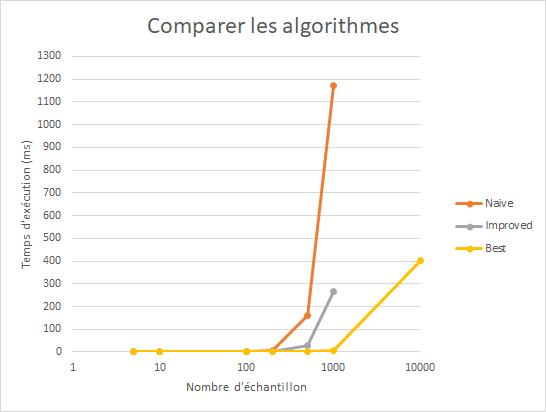
\includegraphics[width=0.8\linewidth]{img/P1_time.png}
    \caption{Graphe de temps d'exécution}
\end{figure}

\clearpage

Nous voyons clairement que l'algorithme \emph{Best} donne la solution le plus rapidement quand le volume des données est énorme. Nous ajoutons ici quelques visualisations (figures \ref{L'arbre le plus court lorsque $N=5$}, \ref{L'arbre le plus court lorsque $N=10$}, \ref{L'arbre le plus court lorsque $N=100$}) de jeux données et le réseau trouvé (le code de visualisation, écrit en MATLAB dans le fichier plot.m est en annexe).

\begin{figure}[!ht]
    \centering
    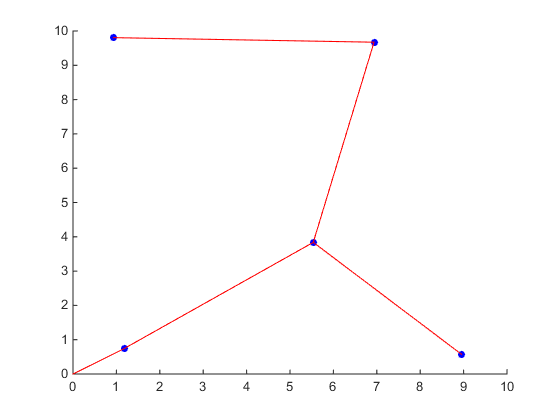
\includegraphics[width=0.8\linewidth]{img/n=5_maxX=10_maxY=10.png}
    \caption{L'arbre le plus court lorsque $N=5$}
    \label{L'arbre le plus court lorsque $N=5$}
\end{figure}

\begin{figure}[!ht]
    \centering
    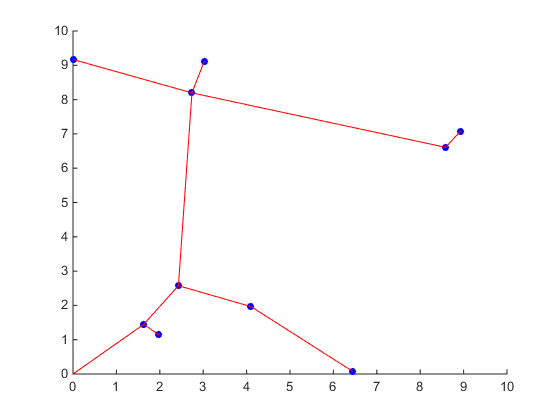
\includegraphics[width=0.8\linewidth]{img/n=10_maxX=10_maxY=10.png}
    \caption{L'arbre le plus court lorsque $N=10$}
    \label{L'arbre le plus court lorsque $N=10$}
\end{figure}

\begin{figure}[!ht]
    \centering
    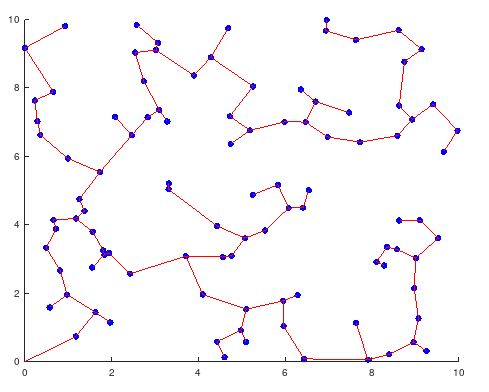
\includegraphics[width=0.8\linewidth]{img/n=100_maxX=10_maxY=10.png}
    \caption{L'arbre le plus court lorsque $N=100$}
    \label{L'arbre le plus court lorsque $N=100$}
\end{figure}

\section{Plannification de production d'huiles}

\subsection{Modèle 1}
Soient les paramètres:
\begin{itemize}
    \item $V$: l'ensemble des huiles végétales brutes.
    \item $H$: l'ensemble des huiles hydrogénées brutes.
    \item $B = V \cup H$: l'ensemble des huiles brutes.
    \item $N$: le nombre de mois à planifier.
    \item $p_f$: prix de vente du produit final. (euro/t)
    \item $p_{i,j}$: coût d'achat de l'huile $i$ au mois $j$. (euro/t)
    \item $V_{max}$: quantité maximale de raffinage d'huiles végétales. (t)
    \item $H_{max}$: quantité maximale de raffinage d'huiles hydrogénées. (t)
    \item $SM_i$: stock maximal chaque mois pour l'huile $i$. (t)
    \item $c_s$: coût de stockage. (euro/t)
    \item $SI_i$: stock initial de l'huile $i$. (t)
    \item $SF_i$: stock final de l'huile $i$. (t)
    \item $v_i$: coefficient de viscosité de l'huile $i$.
    \item $v_{min}$: viscosité minimale du produit final.
    \item $v_{max}$: viscosité maximale du produit final.
\end{itemize}

Soient les variables:
\begin{itemize}
    \item $a_{i,j}$: quantité d'achat de l'huile $i$ au mois $j$. (t)
    \item $s_{i,j}$: stock de l'huile $i$ au mois $j$. (t)
    \item $r_{i,j}$: quantité de raffinage de l'huile $i$ au mois $j$. (t)
\end{itemize}

Soit $P$ le profit de l'entreprise après $N$ mois.

Le système d'équations linéaires (la fonction objective avec les contraintes) est décrite de la manière suivante:
\begin{align*}
    & \text{Maximizer } P = \sum\limits_{j = 1}^N {\sum\limits_{i \in B}^{} {{r_{i,j}}p_f} }  - \sum\limits_{j = 1}^N {\sum\limits_{i \in B}^{} {{a_{i,j}}{p_{i,j}}} }  - {c_s}\sum\limits_{j = 1}^N {\sum\limits_{i \in B}^{} {{s_{i,j}}} }\\
    & \text{Sous contraintes : }\\
    & \forall j = \overline {1,N} :\sum\limits_{i \in V}^{} {{r_{i,j}}}  \le {V_{\max }}\\
    & \forall j = \overline {1,N} :\sum\limits_{i \in H}^{} {{r_{i,j}}}  \le {H_{\max }}\\
    & \forall j = \overline {1,N} :\sum\limits_{i \in B}^{} {{r_{i,j}}{v_i}}  \le {v_{\max }}\sum\limits_{i \in B}^{} {{r_{i,j}}} \\
    & \forall j = \overline {1,N} :\sum\limits_{i \in B}^{} {{r_{i,j}}{v_i}}  \ge {v_{\min }}\sum\limits_{i \in B}^{} {{r_{i,j}}} \\
    & \forall j = \overline {1,N} ,\forall i \in B:{s_{i,j}} = {s_{i,j - 1}} + {a_{i,j}} - {r_{i,j}}\\
    & \forall i \in B:{s_{i,0}} = S{I_i}\\
    & \forall i \in B:{s_{i,N}} = S{F_i}\\
    & \forall j = \overline {0,N} ,\forall i \in B:S{M_i} \ge {s_{i,j}} \ge 0;{a_{i,j}} \ge 0;{r_{i,j}} \ge 0
\end{align*}

La solution sera affichée comme ceci dans le fichier
"OilFabrication/OilFab\_{}a.res" :
\begin{itemize}
    \item Le profit maximal après $N$ mois: $P$ (euros).
    \item Au mois $j$:
    \begin{itemize}
        \item Pour l'huile $i$:
        \begin{itemize}
            \item Achater : $a_{i,j}$ tonne(s).
            \item Raffiner : $r_{i,j}$ tonne(s).
            \item Stocker : $s_{i,j}$ tonne(s).
        \end{itemize}
    \end{itemize}
\end{itemize}

On obtient un profit maximal après 6 mois de \textbf{107843} (euros).

\subsection{Modèle 2}
Soient les paramètres:
\begin{itemize}
    \item $V$: l'ensemble des huiles végétales brutes.
    \item $H$: l'ensemble des huiles hydrogénées brutes.
    \item $B = V \cup H$: l'ensemble des huiles brutes.
    \item $N$: le nombre de mois à planifier.
    \item $p_f$: prix de vente du produit final. (euro/t)
    \item $p_{i,j}$: coût d'achat de l'huile $i$ au mois $j$. (euro/t)
    \item $V_{max}$: quantité maximale de raffinage d'huiles végétales. (t)
    \item $H_{max}$: quantité maximale de raffinage d'huiles hydrogénées. (t)
    \item $SM_i$: stock maximal chaque mois de l'huile $i$. (t)
    \item $c_s$: coût de stockage. (euro/t)
    \item $SI_i$: stock initial de l'huile $i$. (t)
    \item $SF_i$: stock final de l'huile $i$. (t)
    \item $v_i$: coefficient de viscosité de l'huile $i$.
    \item $v_{min}$: viscosité minimale de produit final.
    \item $v_{max}$: viscosité maximale de produit final.
    \item $D = B \times B$: couples de dépendances. $(x, y) \in D$ signifie que si $x$ est utilisée, $y$ doit être utilisée aussi.
    \item $n_{max}$: nombre maximal d'huiles utilisées dans un mois.
    \item $u_{min}$: la quantité minimale si une huile est utilisée. (t)
    \item $M = V_{max} + H_{max}$: un grand nombre.
\end{itemize}

Soient les variables:
\begin{itemize}
    \item $a_{i,j}$: quantité d'achat de l'huile $i$ au mois $j$. (t)
    \item $s_{i,j}$: stock de l'huile $i$ au mois $j$. (t)
    \item $r_{i,j}$: quantité de raffinage de l'huile $i$ au mois $j$. (t)
    \item $u_{i,j}$: variable binaire, indiquant l'usage de l'huile $i$ au mois $j$.
\end{itemize}

Soit $P$ le profit de l'entreprise après $N$ mois.

Le système d'équations linéaires (la fonction objective avec les contraintes) est décrit de la manière suivante:
\begin{align*}
    & \text{Maximizer } P = \sum\limits_{j = 1}^N {\sum\limits_{i \in B}^{} {{r_{i,j}}p_f} }  - \sum\limits_{j = 1}^N {\sum\limits_{i \in B}^{} {{a_{i,j}}{p_{i,j}}} }  - {c_s}\sum\limits_{j = 1}^N {\sum\limits_{i \in B}^{} {{s_{i,j}}} }\\
    & \text{Sachant que : }\\
    & \forall j = \overline {1,N} :\sum\limits_{i \in V}^{} {{r_{i,j}}}  \le {V_{\max }}\\
    & \forall j = \overline {1,N} :\sum\limits_{i \in H}^{} {{r_{i,j}}}  \le {H_{\max }}\\
    & \forall j = \overline {1,N} :\sum\limits_{i \in B}^{} {{r_{i,j}}{v_i}}  \le {v_{\max }}\sum\limits_{i \in B}^{} {{r_{i,j}}} \\
    & \forall j = \overline {1,N} :\sum\limits_{i \in B}^{} {{r_{i,j}}{v_i}}  \ge {v_{\min }}\sum\limits_{i \in B}^{} {{r_{i,j}}} \\
    & \forall j = \overline {1,N} ,\forall i \in B:{s_{i,j}} = {s_{i,j - 1}} + {a_{i,j}} - {r_{i,j}}\\
    & \forall i \in B:{s_{i,0}} = {SI_i}\\
    & \forall i \in B:{s_{i,N}} = {SF_i}\\
    & \forall j = \overline {1,N} ,\forall i \in B:{u_{\min }}*{u_{i,j}} \le {r_{i,j}} \le M*{u_{i,j}}\\
    & \forall j = \overline {1,N} :\sum\limits_{i \in B}^{} {{u_{i,j}}}  \le {n_{\max }}\\
    & \forall j = \overline {1,N} ,\forall \left( {{i_1},{i_2}} \right) \in D:{u_{{i_1},j}} \le {u_{{i_2},j}}\\
    & \forall j = \overline {0,N} ,\forall i \in B:S{M_i} \ge {s_{i,j}} \ge 0;{a_{i,j}} \ge 0;{r_{i,j}} \ge 0
\end{align*}

La solution sera affichée comme ceci dans le fichier
"OilFabrication/OilFab\_{}b.res" :
\begin{itemize}
    \item Le profit maximal après $N$ mois: $P$ (euros).
    \item Au mois $j$:
    \begin{itemize}
        \item Pour l'huile $i$ (si utilisée):
        \begin{itemize}
            \item Achater : $a_{i,j}$ tonne(s).
            \item Raffiner : $r_{i,j}$ tonne(s).
            \item Stocker : $s_{i,j}$ tonne(s).
        \end{itemize}
    \end{itemize}
\end{itemize}

On obtient un profit maximal après 6 mois de \textbf{100279} (euros).

\section{Annexe}

\subsection{Visualisation d'arbre (plot.m)}

\lstinputlisting[language=Matlab]{ShortestSpanningTree/plots.m}
\end{document}